\documentclass[10pt,twocolumn,letterpaper]{article}

\usepackage{iccv}
\usepackage{times}
\usepackage{epsfig}
\usepackage{graphicx}
\usepackage{amsmath}
\usepackage{amssymb}

% Include other packages here, before hyperref.

% If you comment hyperref and then uncomment it, you should delete
% egpaper.aux before re-running latex.  (Or just hit 'q' on the first latex
% run, let it finish, and you should be clear).
\usepackage[breaklinks=true,bookmarks=false]{hyperref}

\iccvfinalcopy % *** Uncomment this line for the final submission

\def\iccvPaperID{****} % *** Enter the ICCV Paper ID here
\def\httilde{\mbox{\tt\raisebox{-.5ex}{\symbol{126}}}}

% Pages are numbered in submission mode, and unnumbered in camera-ready
\ificcvfinal\pagestyle{empty}\fi

\begin{document}

%%%%%%%%% TITLE
\title{Neural Network Regression with Handwritten Characters}

\author{Kotaro Tachibana\\
Tokyo Institute of Technology\\
Tokyo, Japan\\
{\tt\small tachibana.k.ae@m.titech.ac.jp}
}

\maketitle
% Remove page # from the first page of camera-ready.
\ificcvfinal\thispagestyle{empty}\fi

%%%%%%%%% ABSTRACT
\begin{abstract}
    In this paper, I estimated the writing time using handwritten character images, and compared the scores using the models in the Pytorch subpackag as regression models.
    In addition, I estimated the writing time for the different character from the training.
    As a result, It was found that the model were not able to learn the characteristics of the characters written quickly or slowly across character types.
\end{abstract}

%%%%%%%%% BODY TEXT
\section{Introduction}

Classification is a well-known problem
that can be solved by deep learning,
but deep learning is also useful for regression problems.
For example, groundwater potential maps can be estimated from map image data \cite{panahi2020spatial} and
right ventricle (RV) can be segmented from cardiac magnetic resonance (MR) images \cite{chen2018correlated}
by neural network regression model.
Existing neural network models for classification can be used for regression with a little modification.
In this report, I estimated the writing time from handwritten characters.

\section{Dataset}
I prepared a dataset of handwritten kanji character "Sho" images and their writing time pairs.
As shown in the Fig.\ref{fig:sho}, I prepared 20 sheets each of fast-written Kanji characters and slow-written Kanji characters.
80\% of each data was used for training and 20\% for validation.
The training data was increased by a factor of 5 using data augmentation with random rotation.
Therefore, the neural network model needs to learn the features that appear when the kanji character "sho" is written quickly and when it is written slowly.
\begin{figure}[h]
    \begin{center}
        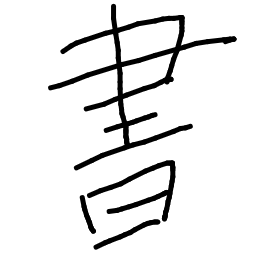
\includegraphics[width=0.4\linewidth]{images/U66F8_00003.png}
        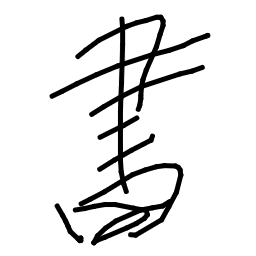
\includegraphics[width=0.4\linewidth]{images/U66F8_00030.png}
    \end{center}
    \caption{Left: "Sho" written late, Right: "Sho" written early}
    \label{fig:sho}
\end{figure}

\section{Model selection}
The neural network model used was a subpackage of Pytorch: \url{https://pytorch.org/docs/stable/torchvision/models.html}.
The subpackage include well-known neural network models such as DenseNet \cite{huang2017densely} and ResNet \cite{he2016deep}.
I repeatedly trained and evaluated using these models.
These models are built for ImageNet in a subpackage with an output size of 1000.
Therefore, it can be trained as a regression model with an output size of 1.

\section{Learning and Evaluation}
The loss function was MSE, and Adadelta \cite{zeiler2012adadelta} was used for optimization.
The best MAE of the model is the minimum MAE at the time of validation after repeated training and validation with 50 epochs. The best MAE was obtained for each model,
and the model with the smallest MAE was selected.

\section{Result}
The best model was Inception v3 \cite{szegedy2016rethinking}.
The MAE for each epoch was Fig. and the best MAE was 224 ms.

\begin{figure}[h]
    \begin{center}
        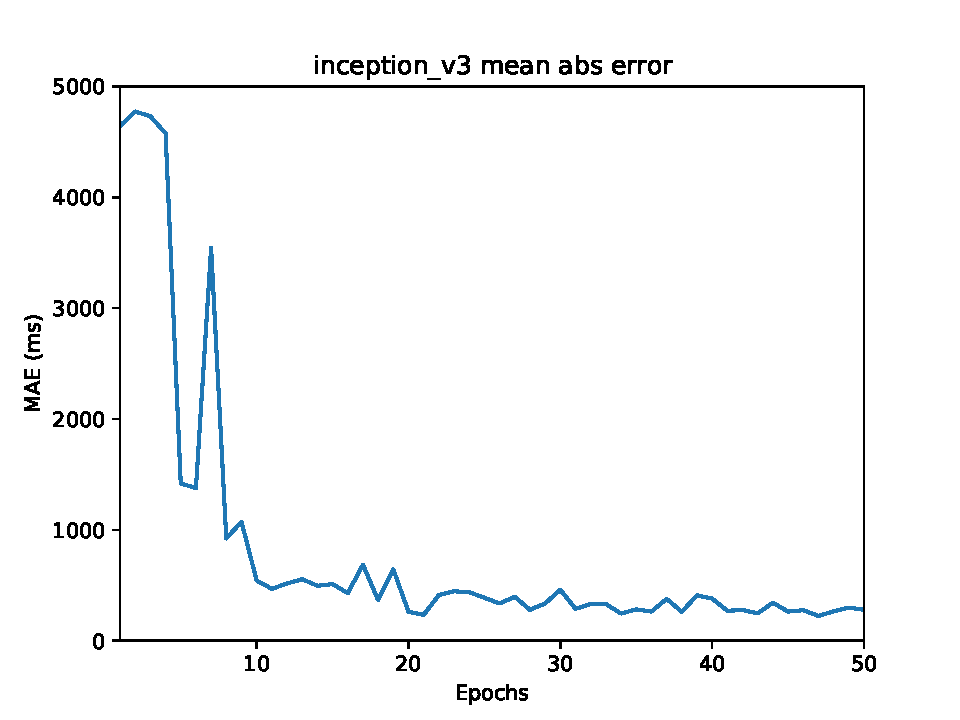
\includegraphics[width=0.8\linewidth]{images/inception_v3.pdf}
    \end{center}
    \caption{Learning curve of the Inception v3 model}
    \label{fig:inception_v3}
\end{figure}

DenseNet161 \cite{huang2017densely} Fig.\ref{fig:densenet161}, ResNet50 \cite{he2016deep} Fig.\ref{fig:resnet50}, and ShuffleNet v2 \cite{ma2018shufflenet} Fig.\ref{fig:shufflenet} were also excellent models
with best MAE of less than 300 ms, which is as good as Inception v3.

\begin{figure}[h]
    \begin{center}
        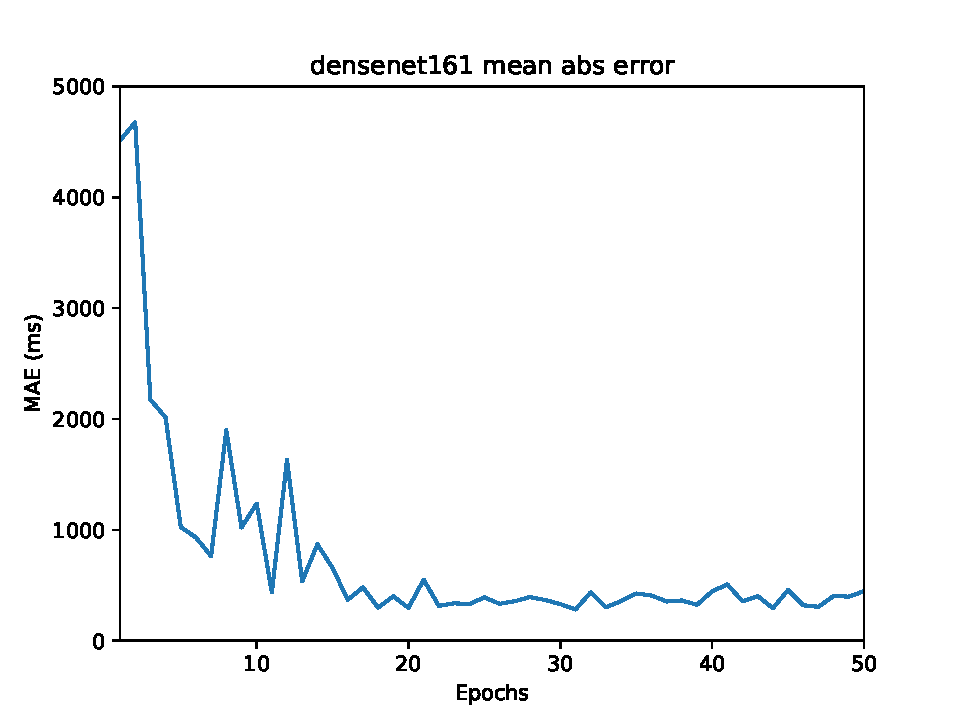
\includegraphics[width=0.8\linewidth]{images/densenet161.pdf}
    \end{center}
    \caption{Learning curve of the DenseNet161 model}
    \label{fig:densenet161}
\end{figure}

\begin{figure}[h]
    \begin{center}
        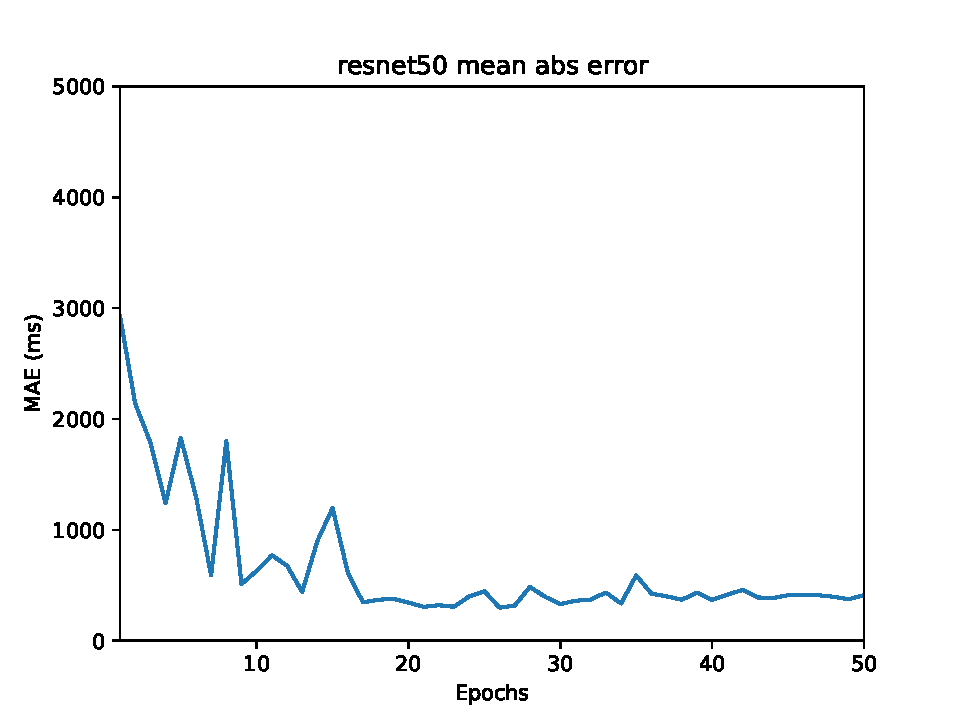
\includegraphics[width=0.8\linewidth]{images/resnet50.pdf}
    \end{center}
    \caption{Learning curve of the ResNet50 model}
    \label{fig:resnet50}
\end{figure}

\begin{figure}[h]
    \begin{center}
        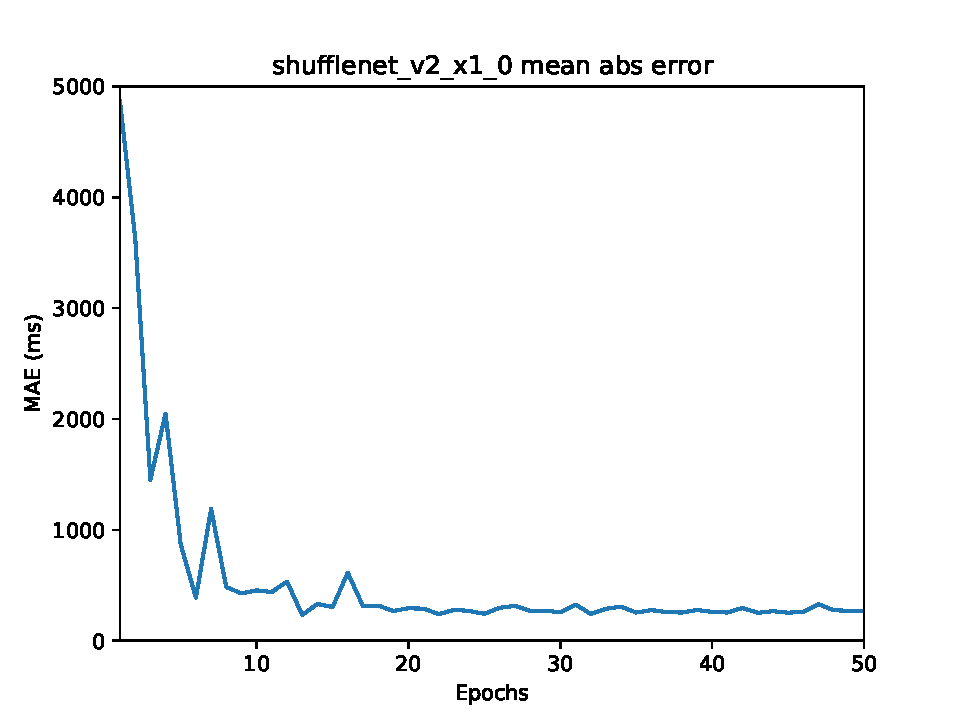
\includegraphics[width=0.8\linewidth]{images/shufflenet_v2_x1_0.pdf}
    \end{center}
    \caption{Learning curve of the ShuffleNet v2 model}
    \label{fig:shufflenet}
\end{figure}

\section{Estimate another character}
In addition, I tried to estimate the writing time of different letters from the learning time.
The image of "Sho" was used for training, and the character "Dou" was used for validation.
As shown in Fig.\ref{fig:dou} ,I prepared two versions of "Dou", one written early and one written late, just like "Sho".
On the other hand, I used "Dou" for training and "Sho" for validation,
or used both "Sho" and "Dou" for training,
and so on for all the previous 9 patterns (3x3).
The model was Inception v3, and the epoch number, loss function, optimization,
and data augmentation were done in the same way.

\begin{figure}[h]
    \begin{center}
        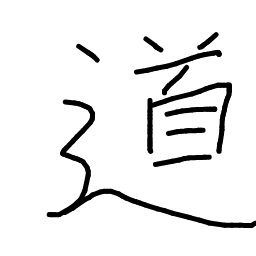
\includegraphics[width=0.4\linewidth]{images/U9053_00002.png}
        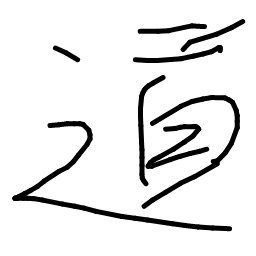
\includegraphics[width=0.4\linewidth]{images/U9053_00034.png}
    \end{center}
    \caption{Left: "Dou" written late, Right: "Dou" written early}
    \label{fig:dou}
\end{figure}

\section{Result of estimation another character}
The results are shown in Table.\ref{table:result_matrix}.
The MAE exceeds 1 second for the validation of different characters from the training.
The learning curve is shown as Fig\ref{fig:sho_dou}.
It was found that the model were not able to learn the characteristics of the characters written quickly or slowly across character types.

\begin{table}[h]
    \begin{center}
        \begin{tabular}{|c|c|ccc|}\hline
            \multicolumn{2}{|c|}{} & \multicolumn{3}{c|}{Training}                             \\
            \cline{3-5}
            \multicolumn{2}{|c|}{} & Sho                           & Dou  & Sho and Dou        \\ \hline
                                   & Sho                           & 224  & 1999        & 1633 \\
            Validation             & Dou                           & 1592 & 366         & 1416 \\
                                   & Sho and Dou                   & 651  & 551         & 687  \\ \hline
        \end{tabular}
    \end{center}
    \caption{Result matrix of estimation}
    \label{table:result_matrix}
\end{table}

\begin{figure}[h]
    \begin{center}
        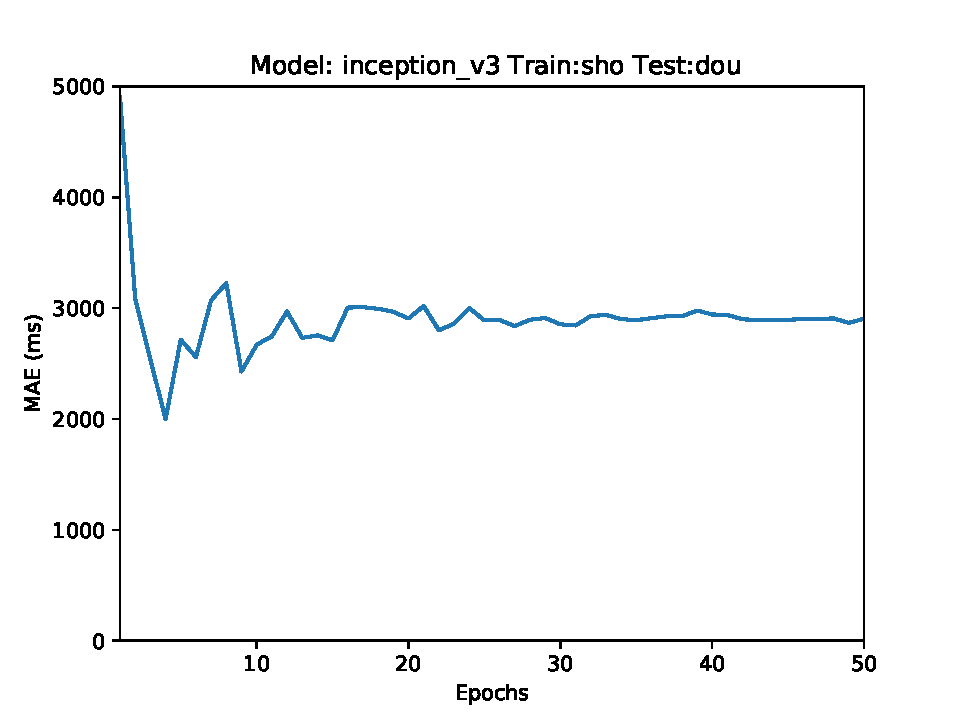
\includegraphics[width=0.8\linewidth]{images/inception_v3_sho_dou.pdf}
    \end{center}
    \caption{Learning curve of "Sho" during training and "Dou" during validation}
    \label{fig:sho_dou}
\end{figure}

\section{Conclusion}
In this report, I estimated the writing time using handwritten character images.
The Inception v3 model scored the best by comparison using the Pytorch subpackage.
The error when estimating the same characters as in training was about 200 ms,
but when estimating different characters from training, the error exceeded 1 second.
I found that it was difficult to learn the universal characteristics of fast and slow writing across letter types.

    {\small
        \bibliographystyle{ieee_fullname}
        \bibliography{egbib}
    }

\end{document}
